\documentclass[12pt,a4paper]{article}
\usepackage{adjustbox} % in preamble

\usepackage[utf8]{inputenc}
\usepackage[latvian]{babel}
\usepackage{caption}
\usepackage{hyperref}

% Make captions "1. attēls."
\DeclareCaptionLabelFormat{numberfirst}{\arabic{figure}. attēls}
\captionsetup[figure]{labelformat=numberfirst,labelsep=period}

% Command for referencing: "1. attēls"
\newcommand{\figref}[1]{\ref{#1} attēls}


\pagenumbering{arabic} % Sets page numbering to arabic (1, 2, 3, ...)
\setcounter{page}{1} % Specifies the starting page number

\usepackage{tabularx} % in your preamble
\usepackage{amsmath, amssymb}
\usepackage{graphicx}
\usepackage{geometry}
\usepackage{subcaption}
\usepackage{float}
\usepackage{array}
\usepackage{booktabs}
\usepackage{enumitem}
\usepackage{fancyhdr}
\usepackage{xcolor}
\usepackage{framed}
\usepackage{titlesec}

% Example 1: Bold, larger font, with some vertical spacing
\titleformat{\section}
  {\normalfont\Large\bfseries} % format: font + weight
  {\thesection}                % label (number)
  {0.3em}                         % space between number and title
  {}                            % code before title text

\geometry{
    left=2cm,
    right=2cm,
    top=2.5cm,
    bottom=2.5cm
}

\pagestyle{plain}
\fancyhf{}
\rhead{Olbaltumvielas}

% Custom colors and environments
\definecolor{taskbg}{rgb}{0.95,0.95,0.95}

% Custom environment for tasks
\newenvironment{taskbox}
{\begin{framed}\begin{minipage}{\textwidth}}
{\end{minipage}\end{framed}}

\title{\textbf{Tests par gremošanu}}
\author{}
\date{}

\begin{document}

\maketitle


\noindent \textbf{1. jautājums.} Kura līkne atbilst kura enzīma aktivitātei dažādos pH \ref{fig:liknes} attēlā? Dotie enzīmi: amilāze, pepsīns, tripsīns.

\begin{figure}[H]
    \centering
    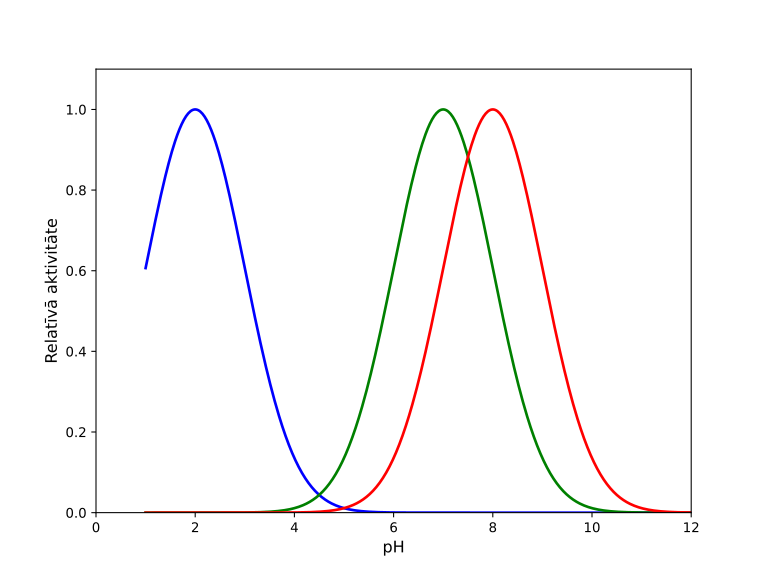
\includegraphics[width=0.5\textwidth]{atteli/enzimi_pH.png}
    \caption{Enzīmu aktivitātes.}
    \label{fig:liknes}
\end{figure}

\noindent \textbf{2. jautājums.} Kurš hormons izdalās no kuņģa sieniņām, kad ēdiens tās stiepj? 

\begin{enumerate}[label=\Alph*.]
    \item gastrīns
    \item pepsīns
    \item insulīns
    \item glikagons
\end{enumerate}

\noindent \textbf{3. jautājums.} Kā hormoni kontrolē cukura līmeni asinīs? 

\begin{enumerate}[label=\Alph*.]
    \item Insulīns paaugstina un glikagons samazina, izraisot glikozes absorbciju.
    \item Insulīns paaugstina un glikagons samazina, izraisot glikogēna sadalīšanu glikozē.
    \item Insulīns samazina un glikagons paaugstina, izraisot glikogēna sadalīšanu glikozē.
    \item Insulīns samazina un glikagons paaugstina, izraisot glikozes absorbciju.
\end{enumerate}

\noindent \textbf{4. jautājums.} Kā atšķiras cukura diabēta veidi?

\begin{enumerate}[label=\Alph*.]
    \item  1. tipa — šūnu rezistence pret insulīnu, 2. tipa — paaugstināts insulīna līmenis.
    \item 1. tipa — paaugstināts insulīna līmenis, 2. tipa — šūnu rezistence pret insulīnu. 
    \item 1. tipa — šūnu rezistence pret insulīnu, 2. tipa — pazemināts insulīna līmenis. 
    \item 1. tipa — pazemināts insulīna līmenis, 2. tipa — šūnu rezistence pret insulīnu. 
\end{enumerate}

\noindent \textbf{5. jautājums.} Kā kuņģa šūnas nodrošina olbaltumvielu gremošanu? 

\begin{enumerate}[label=\Alph*.]
    \item Parietālās šūnas izdala pepsinogēnu, kurš pārveidojas par pepsīnu $H^+$ un $Cl^-$ klātbūtnē, kurus izdala galvenās šūnas.
    \item Galvenās šūnas izdala pepsinogēnu, kurš pārveidojas par pepsīnu $H^+$ un $Cl^-$ klātbūtnē, kurus izdala parietālās šūnas. % Correct answer
    \item Parietālās šūnas izdala pepsinogēnu, kurš pārveidojas par pepsīnu $H^+$ un $CO_3^{-}$ klātbūtnē, kurus izdala galvenās šūnas.
    \item Galvenās šūnas izdala pepsinogēnu, kurš pārveidojas par pepsīnu $H^+$ un $CO_3^{-}$ klātbūtnē, kurus izdala parietālās šūnas.
\end{enumerate}

\noindent \textbf{6. jautājums.} Kā hormoni kontrolē ēstgribu?

\begin{enumerate}[label=\Alph*.]
    \item Supresori: insulīns, leptīns, PYY. Stimulanti: grelīns. 
    \item Supresori: insulīns, leptīns. Stimulanti: grelīns, PYY.
    \item Supresori: insulīns. Stimulanti: grelīns, PYY, leptīns.
    \item Supresori: insulīns, grelīns, PYY. Stimulanti: leptīns.
\end{enumerate}

\noindent \textbf{7. jautājums.} Kad hīms (barības putriņa) nonāk divpadsmitpirkstu zarnā, tā izdala hormonus holecistokinīnu un sekretīnu. Kurš apgalvojums pareizi raksturo to hormonālo kontroli? 

\begin{enumerate}[label=\Alph*.]
    \item Tie stimulē kuņģa sfinktera relaksāciju.
    \item Tie inhibē vielu sekrēciju kuņģī.
    \item Tie stimulē vielu sekrēciju no aizkuņģa dziedzera un žultspūšļa un inhibē peristaltiku.
    \item Tie stimulē kuņģa pH neitralizēšanu.
\end{enumerate}

\noindent \textbf{8. jautājums.} Žults sāļi sadala taukus mazākos pilienos un lipāze sadala triglicerīdus monoglicerīdos un taukskābēs. Kurā orgānā notiek šis process? 

\begin{enumerate}[label=\Alph*.]
    \item divpadsmitpirkstu zarnā
    \item tievajā zarnā
    \item aklajā zarnā
    \item resnajā zarnā
\end{enumerate}

\noindent \textbf{9. jautājums.} Kurš no enzīmiem nepiedalās gremošanas procesā tievajā zarnā

\begin{enumerate}[label=\Alph*.]
    \item maltāze
    \item nukleāze
    \item tripsīns
    \item pepsīns
\end{enumerate}

\noindent \textbf{10. jautājums.} Kāda ir atgremotāju gremošanas orgānu secība? 
\begin{enumerate}[label=\Alph*.]
    \item glumenieks, spureklis, aceknis, grāmatnieks
    \item  spureklis, aceknis, grāmatnieks, glumenieks
    \item aceknis, grāmatnieks, glumenieks, spureklis
    \item grāmatnieks, glumenieks, spureklis, aceknis
\end{enumerate}


\section*{Atsauces}
\begin{enumerate}[leftmargin=*]
    \item Atgremotāju shēma: \url{vegan.lv}
\end{enumerate}


\newpage
\section*{Atbildes}

\begin{enumerate}
\item C. Pepsīns izdalās kuņģī, kur zemais pH atvieglo proteīnu šķelšanu aminoskābēs. Siekalu amilāze izdalās mutē, kura ir aptuveni neitrāla. Tripsīns darbojas tievajā zarnā, kur pH ir nedaudz bāzisks $HCO_3^{-}$.
\item A. Gastrīns tiek izdalīts, cirkulē asinsritē un stimulē parietālās kuņģa šūnas, kuras izdala kuņģa skābi. Pepsīns nav hormons. Insulīns un glikagons tiek izdalīts cukura līmeņa maiņu rezultātā.
\item C.
\item D.
\item B. 
\item A. Leptīnu izdala taukaudi. Kad taukaudu daudzums samazinās, leptīna līmeņi samazinās un ir lielāka ēstgriba. Tievā zarna izdala PYY – antagonistu grelīnam. Grelīnu izdala ķunģa sieniņas.
\item C. Peristaltika tiek inhibēta liela tauku satura gadījumā. Lēna peristlatika nodrošina efektīvu tauku sagremošanu.
\item B.
\item D. Pepsīns nav aktīvs tievās zarnas neitrālajā pH.
\item B. Pirmajā kārtā barību apstrādā spureklis un aceknis, tad tā tiek atgremota un sakošļāta līdz beidot nonāk grāmatniekā un glumeniekā (\figref{fig:atgremotajs})
\end{enumerate}

\begin{figure}[H]
    \centering
    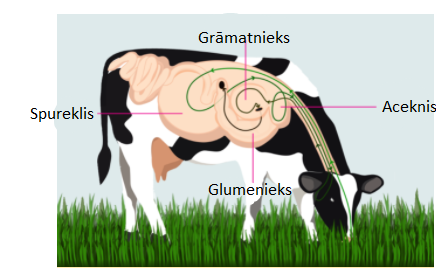
\includegraphics[width=0.5\textwidth]{atteli/atgremotajs.png}
    \caption{Atgremotāju gremošanas sistēma.}
    \label{fig:atgremotajs}
\end{figure}

\end{document}